\section{Ecuaciones Especiales de Primer Orden}

{}
  Cualquier ecuación diferencial de primer orden de la \emph{forma normal}
     \begin{align*}
   \dfrac{dy}{dx} = f(x,y)
   \end{align*}
   puede ser reescrita en la \emph{forma diferencial}
       \begin{align*}
    M(x,y)dx+N(x,y)dy =0
    \end{align*} 
    y  viceversa. 

%%%%%%%%%%%%%%%%%%%%%
{Separación de variables}
Una ecuación es \emph{separable} si se puede escribir en la forma. 
 \begin{align*}
 f_{1}(x)g_{1}(y)dx+f_{2}(x)g_{2}(y)dy = 0
 \end{align*}
 
%%%%%%%%%%%%%%%%%%%%%
{}
En ese caso, su solución  está dada por
   \begin{align*}
       \displaystyle \int \dfrac{f_{1}(x)}{f_{2}(x)}dx
       + \int \dfrac{g_{2}(y)}{g_{1}(y)}dy = c
  \end{align*}
  siempre que $g_{1}(y)f_{2}(x)\neq 0$.

%%%%%%%%%%%%%%%%%%%%%

	\begin{problema}
		Resuelve la ecuación diferencial
		\begin{align*}
		xdy-ydx=0
		\end{align*}
	\end{problema}

{Ecuaciones exactas}
  Una ecuación
     \begin{align*}
   M(x,y)dx + N(x,y)dy = 0
   \end{align*}
   es \emph{exacta} si 
   existe una función diferenciable $U:\R^{2}\to \R$ tal que
       \begin{align*}
       M(x,y)dx + N(x,y)dy = dU(x,y) = 0 
    \end{align*}
 

En ese caso, la solución está dada por                                         \begin{align*}
U(x,y) = c
\end{align*}

%%%%%%%%%%%%%%%%%%%%%
{}
Un criterio para determinar si una ecuación es exacta es verificar que 
\begin{align*}
    \dfrac{\partial M}{\partial y}= \dfrac{\partial N}{\partial x}
    \end{align*}

%%%%%%%%%%%%%%%%%%%%%

	\begin{problema}
		Determina si la ecuación
		\begin{align*}
			xdy-ydx=0
		\end{align*}
		es exacta.
	\end{problema}

{}
  De manera equivalente, podemos encontrar la solución de la siguiente manera 
  \begin{align*}
   \displaystyle \int M\partial x+ \int \left( N - \dfrac{\partial }{\partial y}\int M\partial x \right)dy = c
   \end{align*}
   
   donde \emph{$\partial x$} indica que la integración es realizada únicamente respecto a $x$, manteniendo $y$ constante. 

%%%%%%%%%%%%%%%%%%%%%

	\begin{problema}
		Demuestra que la ecuación
		\begin{align*}
		\dfrac{xdy-ydx}{x^2}=0
		\end{align*}
		es exacta y resuélvela. 
	\end{problema}

{Factor Integrante}
  Cuando una ecuación no es exacta, en ocasiones se puede encontrar de manera explícita una función $\mu:\R^{2}\to \R$ llamada \emph{factor integrante} tal que 
\begin{align*}
 \dfrac{\partial }{\partial y}\left( \mu M \right) = 
 \dfrac{\partial }{\partial x}\left( \mu N \right)
 \end{align*}
 
 y por tanto 
 \begin{align*}
  \mu M dx + \mu N dy = 0
  \end{align*}
  es exacta.

%%%%%%%%%%%%%%%%%%%%%
{}
  \begin{figure}
 \centering
 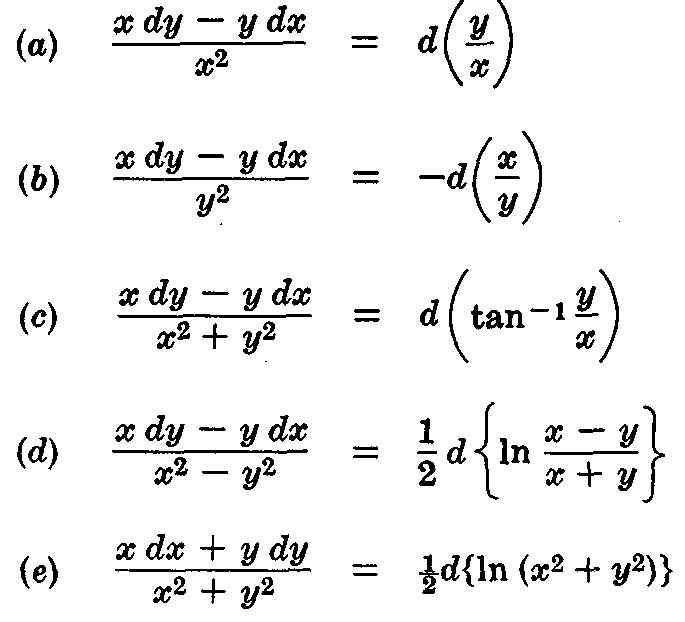
\includegraphics[height=.6\textheight,keepaspectratio=true]{./edo/factores_integrantes_usuales.png}
 % factores_integrantes_usuales.png: 685x622 px, 96dpi, 18.12x16.46 cm, bb=0 0 514 466
 \caption{Algunos ejemplos de factores integrantes.}
 \label{fig:factores_integrantes_usuales}
\end{figure}


%%%%%%%%%%%%%%%%%%%%%
\subsection{Ecuaciones lineales}
{}
  Diremos que una ecuación es lineal si se puede reescribir en la forma:
  \begin{align*}
   \dfrac{dy}{dx} + p(x)y=q(x)
   \end{align*}

%%%%%%%%%%%%%%%%%%%%%
{}
  En este caso, un factor integrantes está dado por 
  \begin{align*}\displaystyle 
   \mu = e^{\int p(x)dx} 
   \end{align*}
   y la ecuación se puede reescribir como
   \begin{align*}
    \dfrac{d}{dx}\left( \mu y  \right) = \mu q(x)
    \end{align*}

%%%%%%%%%%%%%%%%%%%%%
{}
  Entonces, 
  \begin{align*}\displaystyle 
   \mu y = \int \mu q(x) dx +c
   \end{align*}
   y la solución está dada por 
   \begin{align*}\displaystyle 
    y & = e^{-\int pdx}\left( \int e^{\int p dx} q(x) dx +c \right)\\
    &= e^{-\int pdx}\int e^{\int p dx}  q(x) dx +c e^{-\int pdx}
    \end{align*}

%%%%%%%%%%%%%%%%%%%%%
{}
  \begin{problema}
   Reescribe la ecuación 
   \begin{align*}
    xdy-ydx=0
    \end{align*} en forma lineal;
    calcula el factor integrante y resuelve. 
  \end{problema}


%%%%%%%%%%%%%%%%%%%%%
\subsection{Ecuaciones homogéneas de orden cero}
{}
  Diremos que una ecuación diferencial es \emph{homogénea de orden cero} si se puede reescribir como
\begin{align*}
 \dfrac{dy}{dx}=F\left( \dfrac{y}{x} \right)
 \end{align*}

%%%%%%%%%%%%%%%%%%%%%
{}
  Definimos la variable dependiente $\nu = \dfrac{y}{x}$, de manera que $y = \nu x$.

%%%%%%%%%%%%%%%%%%%%%
{}
  Entonces la ecuación diferencial se puede reescribir como
  \begin{align*}
   v+ x\dfrac{d\nu}{dx}= F(\nu)
   \end{align*}
   o de manera equivalente
   \begin{align*}
    xd\nu + \left( F(\nu)-v \right)dx =0.
    \end{align*}

%%%%%%%%%%%%%%%%%%%%%
{}
  Entonces tiene su solución está dada por 
  \begin{align*}
   \displaystyle 
   \ln |x| = \int \dfrac{d\nu}{F(\nu)-\nu}+c
   \end{align*}

%%%%%%%%%%%%%%%%%%%%%
{}
  \begin{problema}
   Reescriba la ecuación 
   \begin{align*}
    xdy-ydx=0
    \end{align*}
    como una ecuación homogénea de orden cero y resuelva. 
  \end{problema}


%%%%%%%%%%%%%%%%%%%%%
\subsection{Ecuaciones de Bernoulli}
{}
  Diremos que una ecuación es de Bernoulli si se puede reescribir en la forma
  \begin{align*}
   \dfrac{dy}{dx}+p(x)y = q(x)y^{n}
   \end{align*}
   siempre que $n \neq 0,1$

%%%%%%%%%%%%%%%%%%%%%
{}
  En ese caso, hacemos la sustitución $\nu = y^{1-n}$ y la ecuación se reduce a una ecuación lineal, cuya solución está dada por 
  \begin{align*}
  \displaystyle 
   \nu e^{(1-n)\int pdx} = 
   \left( 1-n \right) \int q e^{(1-n)\int pdx}+c
   \end{align*}

%%%%%%%%%%%%%%%%%%%%%
{}
  \begin{observacion}
   \begin{enumerate}[(i)]
     %NUEVO ITEM
     \item Si $n=0$, la ecuación ya es lineal sin necesidad de hacer sustitución alguna. 
     
     \item Si $n=1$, la ecuación se puede reescribir como separable. 
\end{enumerate}
  \end{observacion}


%%%%%%%%%%%%%%%%%%%%%
{}
  \begin{problema}
   Resuelve la ecuación 
   \begin{align*}
    x\dfrac{dy}{dx}+y=xy^{3}
    \end{align*}
  \end{problema}


%%%%%%%%%%%%%%%%%%%%%
\subsection{Ecuaciones solubles}
{}
  Diremos que una ecuación diferencial es soluble para $y$ si 
  \begin{align*}
   y = g\left( x,p \right)
   \end{align*}
   donde $p = y'$.

%%%%%%%%%%%%%%%%%%%%%
{}
  En ese caso, 
  \begin{align*}
   \dfrac{dy}{dx} = \dfrac{dg}{dx}
   = \dfrac{\partial g}{\partial x}+\dfrac{\partial g}{\partial p}\dfrac{\partial p}{\partial x}
   \end{align*}
   
   o de manera equivalente
   \begin{align*}
    p = \dfrac{\partial g}{\partial x}+\dfrac{\partial g}{\partial p}\dfrac{\partial p}{\partial x}
   \end{align*}

%%%%%%%%%%%%%%%%%%%%%
{}
  Resolvemos la ecuación anterior para $p$
  \begin{align*}
   G\left( x,p,c \right)=0
   \end{align*}
   y sustituimos en $y=g(x,p)$.

%%%%%%%%%%%%%%%%%%%%%
{}
  \begin{problema}
   Resuelve la ecuación 
   \begin{align*}
    xp^{2}+2px-y =0
    \end{align*}
    donde $p=y'$.
  \end{problema}


%%%%%%%%%%%%%%%%%%%%%
\subsection{Ecuación de Clairaut}
{}
  Diremos que una ecuación es de Clairaut si se puede reescribir como 
  \begin{align*}
   y = px+F(p)
   \end{align*}
   donde $p = y'$

%%%%%%%%%%%%%%%%%%%%%
{}
  Este es un caso especial del tipo anterior con solución 
  \begin{align*}
   y = cx + F(c)
   \end{align*}

%%%%%%%%%%%%%%%%%%%%%
{}
  \begin{problema}
   Resuelve la ecuación
   \begin{align*}
    y = px\pm \sqrt{p^{2}+1}
    \end{align*}
    donde $p=y'$.
  \end{problema}


%%%%%%%%%%%%%%%%%%%%%
% \subsection{Miscelanea}
% {}
%   Si la ecuación se puede reescribir como
%   \begin{align*}
%    \dfrac{dy}{dx}=F\left( \alpha x +\beta y \right) ,
%    \end{align*} entonces la podemos reducir a una separable con la sustitución 
%    \begin{align*}
%     \nu = \alpha + \beta y
%     \end{align*}
% 
% %%%%%%%%%%%%%%%%%%%%%
% {}
%   Si la ecuación se puede reescribir como 
%   \begin{align*}
%    \dfrac{dy}{dx} = F\left( \dfrac{
%    \alpha_{1}x + \beta_{1} y + \gamma_{1}
%    }{
%    \alpha_{2}x + \beta_{2} y + \gamma_{2}
%    } \right)
%    \end{align*}
% 
% %%%%%%%%%%%%%%%%%%%%%
% {}
%   Si $
%    \dfrac{\alpha_{1}}{\alpha_{2}}\neq \dfrac{\beta_{1}}{\beta_{2}}
%    $, entonces podemos elegir constantes $h,k$ tales que la ecuación se reduce a una homogénea con el cambio de variables
%    \begin{align*}
%     x = X+h, y=Y+k
%     \end{align*}
% 
% %%%%%%%%%%%%%%%%%%%%%
% {}
%   Si $
%    \dfrac{\alpha_{1}}{\alpha_{2}}= \dfrac{\beta_{1}}{\beta_{2}}
%    $,la ecuación se reduce al tipo anterior. 
%   
% 
% %%%%%%%%%%%%%%%%%%%%%
\subsection{Reducción de orden}
{}
  Si una ecuación diferencial es de orden $m>1$, pero hace falta de forma explícita la variable dependiente $y$, entonces se puede reducir de orden con la sustitución 
  $y'=p$.

%%%%%%%%%%%%%%%%%%%%%
{}
  \begin{problema}
   Resuelve la ecuación
   \begin{align*}
    y''+2y'=4x
    \end{align*}
  \end{problema}


%%%%%%%%%%%%%%%%%%%%%
{}
  \begin{problema}
   Resuelve la ecuación 
   \begin{align*}
    1+yy''+y'^{2} = 0
    \end{align*}
  \end{problema}
con la reducción de orden $y'=p$.

%%%%%%%%%%%%%%%%%%%%%
% ejemplos de ecuaciones de primer orden...
% ecuaciones separables
\subsection{Ejemplos}
{}
  \begin{problema}
   \begin{enumerate}[(i)]
     %NUEVO ITEM
     \item Encuentra la solución general de 
     \begin{align*}
      \left( 4x+xy^{2} \right)dx+\left( y+x^{2}y \right)dy = 0
      \end{align*}
     
     \item Encuentra la solución particular para $y(1)=2$.
\end{enumerate}
  \end{problema}


%%%%%%%%%%%%%%%%%%%%%
{}
  Resuelve el problema de valor inicial
  \begin{align*}
   \begin{cases}
\dfrac{dy}{dx}+3y=8 \\
y(0)=2
\end{cases}
   \end{align*}

%%%%%%%%%%%%%%%%%%%%%
{}
  \begin{problema}
   Resuelve la ecuación
   \begin{align*}
    \dfrac{dy}{dx} = \sec(y)\tan(x)
    \end{align*}
  \end{problema}


%%%%%%%%%%%%%%%%%%%%%
% ecuaciones exactas
